\documentclass[12pt]{article}

\title{On the quantum decomposition of the planet Mercury's orbit path}
\author{S. Halayka\footnote{sjhalayka@gmail.com}}
\date{\today\;\currenttime}

\usepackage{datetime}
\usepackage{listings}
\usepackage{cite}
\usepackage{xcolor}
\usepackage{graphicx}
\usepackage{setspace}
\usepackage{amsmath}
\usepackage{url}
\usepackage[margin=1.0in]{geometry}

%\doublespace

%\usepackage[]{lineno}
%\linenumbers


\begin{document}



 
\maketitle

\begin{abstract}
By quantizing the gravitational time dilation using various step sizes, one obtains a set of weighted paths.
The precession associated with each weighted path combines to provide the same answer as the classical analytical solution.
\end{abstract}


\section{Introduction}


\begin{figure} 
\centering
\label{fig4}
  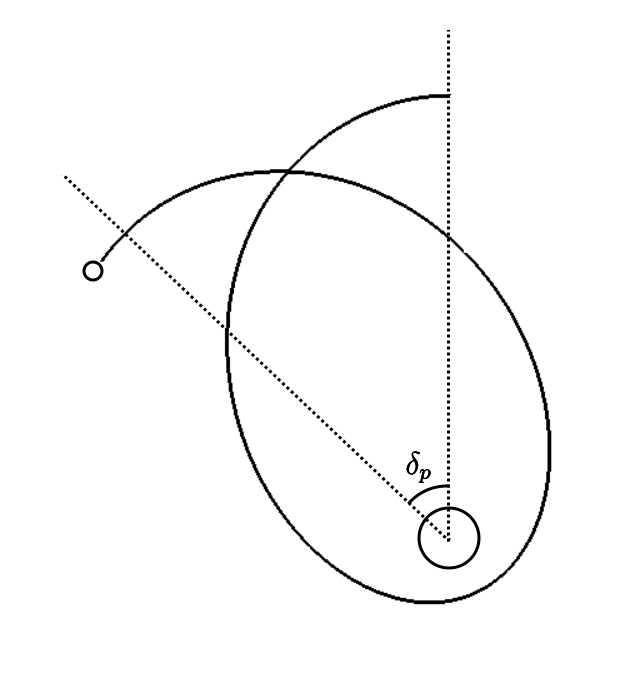
\includegraphics[width = 6 in]{precession.png}
  \caption{ A diagram showing precession, where the orbit does not quite form a closed ellipse.
}
\end{figure}



\begin{thebibliography}{9}


\bibitem{halayka} Halayka. On simulating the four Solar System tests of general relativity using two-parameter post-Newtonian gravitation with Euler integration. (2024)

\end{thebibliography}





\end{document}









